\section{Intégrale de \nom{Gauss}}\label{sec:intGauss}

\begin{marginfigure}[0cm]
    \centering
    % Author: Izaak Neutelings (August, 2017)

% define gaussian pdf and cdf
\pgfmathdeclarefunction{gauss}{3}{%
  \pgfmathparse{1/(#3*sqrt(2*pi))*exp(-((#1-#2)^2)/(2*#3^2))}%
}

% https://tex.stackexchange.com/questions/240642/add-vertical-line-of-equation-x-2-and-shade-a-region-in-graph-by-pgfplots

% plot aspect ratio
%\def\axisdefaultwidth{8cm}
%\def\axisdefaultheight{6cm}

% number of sample points
\def\N{50}

\begin{tikzpicture}[scale=1]
  \message{Cumulative probability^^J}
  
  \def\B{0};
  \def\Bs{6.0};
  \def\xmax{\B+3.5*\Bs};
  \def\ymin{{-0.1*gauss(\B,\B,\Bs)}};
  \def\h{0.07*gauss(\B,\B,\Bs)};
  \def\a{\B-0.8*\Bs};
  
  \begin{axis}[every axis plot post/.append style={
               mark=none,
               domain={-1*(\xmax)}:{1*(\xmax)},samples=\N,smooth},
               % xmin={-1*(\xmax)}, 
               xmax={1.06*(\xmax)},
               ymin=\ymin, ymax={1.3*gauss(\B,\B,\Bs)},
               axis lines=middle,
               axis line style=thick,
               axis line style={-latex},
               ticks=none,
               xlabel=$x$,
               every axis x label/.style={at={(current axis.right of origin)},anchor=north},
               y=700pt,
               clip=false
              ]
    
    % PLOTS
    \addplot[myblue,thick,name path=B] {gauss(x,\B,\Bs)};
    % FILL
    \path[name path=xaxis]
      (0,0) -- (\pgfkeysvalueof{/pgfplots/xmax},0);
    \addplot[mylightblue, opacity=0.9] fill between[of=xaxis and B];
    % LINES
    \node[myblue,above left] at ({-0.7*(\B+\Bs)},{1.2*gauss(\B+\Bs,\B,\Bs)}) {$x \mapsto \mathrm{e}^{-x^2}$};
    \node[myblue] at ({0},{0.6*gauss(0.85*(\a),\B,\Bs)}) {$\sqrt{\pi}$};
    
  \end{axis}
\end{tikzpicture}
    \caption{Intégrale de \nom{Gauss}}
\end{marginfigure}

\begin{theo}
On montre que
\[
\int_0^{+\infty} \e^{-x^2} \d x = \lim_{n\to+\infty} \int_0^{\sqrt{n}} \left(1 - \frac{x^2}{n}\right)^n \d x.
\]

Ainsi,
\begin{equation}\label{eqIntGauss}
        \int_{0}^{+\infty} \e^{-x^2} \d x = \frac{\sqrt{\pi}}{2}        
    \end{equation}
\end{theo}

%-----------œ
\subsection{Calcul de l'intégrale}

\begin{exercice}
\source{\cite{maths-france} Planche no 13. Suites et séries d’intégrales}
On note $I = \int_0^{+\infty} \e^{-x^2} \d x$ et on pose $\fonctionligne[f]{x}{\e^{-x^2}}$.

\begin{questions}
\item Montrer que $I$ est une intégrale convergente.
\end{questions}
On propose ensuite de déterminer la valeur de $I$.
\begin{questions}[resume]
\item \textbf{Première méthode: \say{ à la main }.} \\ 
Pour $n \in \Ne$, on pose
$$
g_n(x) \defeq
\begin{cases}
\left(1 - \frac{x}{n} \right)^n &\text{si } x \in \interff{0}{n} \\
0 &\text{si } x \geqslant n
\end{cases}
$$
puis $\fonctionligne[g]{x}{\e^{-x}}$ et $h_n = g - g_n$.

\begin{questions}
\item Montrer que $h_n$ atteint son maximum sur $\interff{0}{n}$. On notera $x_n$ l'abscisse d'un point en lequel $h_n$ atteint ce maximum.

\item Montrer que $h_n$ est à valeurs positives.

\item Montrer que $h_n(x_n) = \frac{x_n}{n} \e^{-x_n}$.

\item En étudiant la fonction $u \mapsto u \e^{-u}$, en déduire que
\[
\norm{h_n}_\infty \leqslant \frac{1}{n \e}.
\]

\item On pose $I_n= \int_0^{+\infty} g_n(x^2) \d x$. Montrer que $\module{I_n - I} \leqslant \frac{1}{\e \sqrt{n}} + \int_{\sqrt{n}}^{+\infty} \e^{-x^2} \d x$.

\item En déduire le résultat attendu.
\end{questions}

\item \textbf{Deuxième méthode: avec le \theoremeutilise{théorème de convergence dominée}{theo:convergencedominee} et les intégrales de \nom{Wallis}.} \\
On pose $f_n(x) = \left(1 - \frac{x^2}{n}\right)^n \indicatrice{\interfo{0}{\sqrt{n}}}(x)$.
\begin{questions}
\item Montrer que la suite $(f_n)_{n\in\N}$ converge simplement vers $f$.

\item À l'aide du théorème de convergence dominée, en déduire que 
\[
\lim\limits_{n\to+\infty} \int_{\R_+} f_n = \int_0^{+\infty} \e^{-x^2} \d x.
\]
\end{questions}

\item On rappelle que, d'après les résultats sur les intégrales de \nom{Wallis},
\[
\lim_{n\to+\infty} \sqrt{n} \int_0^{\frac{\pi}{2}} \cos(t)^{2n+1} \d t = \frac{\sqrt{\pi}}{2}.
\]

En déduire la valeur de $I$.
\end{questions}
% Pour $n \in \Ne$, on pose
        % $$
        % f_n(x) \defeq
        % \begin{cases}
            % \left(1 - \frac{x^2}{n} \right)^n &\text{si } x \in [0, \sqrt{n}] \\
            % 0 &\text{si } x > \sqrt{n}
        % \end{cases}.
        % $$
        % \begin{enumerate}
            % \item Montrer que la suite $(f_n)_{n \in \Ne}$ converge simplement sur $\Rp$ vers la fonction $f:x \mapsto \e^{-x^2}$.
            % \item À l'aide de la convergence dominée, calculer l'intégrale de \textsc{Gauss}.
        % \end{enumerate}
\end{exercice}

\begin{marginfigure}[-5cm]
    \centering
    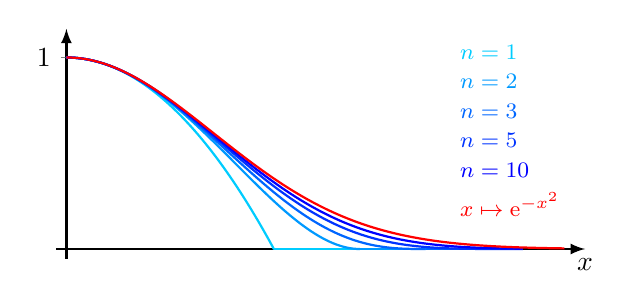
\begin{tikzpicture}
    \begin{axis}[
        width=8.3cm,
        height=4.5cm,        
        xmin=-0.05, xmax=2.5,
        ymin=-0.05, ymax=1.15,
        axis lines=middle,
        axis line style=thick,
        axis line style={-latex},
        legend cell align={left}, 
        legend style={
            draw=none,
            fill=none,
            font=\footnotesize,
            legend image code/.code={\node[anchor=west] {#1};}
        },
        xtick=\empty,
        ytick={0, 1},
        yticklabels={$0$, $1$},
        xlabel=$x$,
        every axis x label/.style={at={(current axis.right of origin)},anchor=north},
    ];

    % Plot for n=1
    \addplot[domain=0:sqrt(1), samples=200, color=blue!20!cyan, smooth, thick, line join=round,line cap=round] {(1 - (x^2)/1)^1};
    \addplot[domain=sqrt(1):2.2, samples=200, color=blue!20!cyan, smooth, thick] {0};
    \addlegendentry{\textcolor{blue!20!cyan}{$n = 1$}}

    % Plot for n=2
    \addplot[domain=0:sqrt(2), samples=200, color=blue!40!cyan, smooth, thick] {(1 - (x^2)/2)^2};
    \addplot[domain=sqrt(2):2.2, samples=200, color=blue!40!cyan, smooth, thick] {0};
    \addlegendentry{\textcolor{blue!40!cyan}{$n = 2$}}

    % Plot for n=3
    \addplot[domain=0:sqrt(3), samples=200, color=blue!60!cyan, smooth, thick] {(1 - (x^2)/3)^3};
    \addplot[domain=sqrt(3):2.2, samples=200, color=blue!60!cyan, smooth, thick] {0};
    \addlegendentry{\textcolor{blue!60!cyan}{$n = 3$}}

    % Plot for n=5
    \addplot[domain=0:2.2, samples=200, color=blue!80!cyan, smooth, thick] {(1 - (x^2)/5)^5};
    \addlegendentry{\textcolor{blue!80!cyan}{$n = 5$}}

    % Plot for n=10
    \addplot[domain=0:2.2, samples=200, color=blue!100!cyan, smooth, thick] {(1 - (x^2)/10)^10};
    \addlegendentry{\textcolor{blue!100!cyan}{$n = 10$}}

    % Plot for exponential function
    \addplot[domain=0:2.4, red, samples=200, smooth, thick] {exp(-x^2)};
    \addlegendentry{\textcolor{red}{$x \mapsto \mathrm{e}^{-x^2}$}}
    \end{axis}
\end{tikzpicture}

    \caption{Illustration de la convergence simple de la suite $(f_n)_{n \in \N}$ vers $f$}
\end{marginfigure}

\begin{solution}
\begin{reponses}
\item La fonction $x \mapsto \e^{-x^2}$ est continue sur $\interfo{0}{+\infty}$. D'après le \theoremeutilise{théorème des croissances comparées}{theo:croissancescomparees}, \mbox{$\e^{-x^2} = \petito_{+\infty}\mathopen{}\left(\frac{1}{x^2}\right)$}. Ainsi, d'après le \theoremeutilise{théorème de comparaison aux intégrales de \nom{Riemann}}{theo:comparaisonintegralesriemann}, la fonction $x \mapsto \e^{-x^2}$ est intégrable sur $\interfo{0}{+\infty}$.

\item
\begin{reponses}
\item Pour tout $x \geqslant n$, $h_n(x) = \e^{-x} \leqslant \e^{-n} = h_n(n)$. De plus, la restriction de la fonction $h_n$ au segment $\interff{0}{n}$ est continue sur ce segment, donc elle y est bornée et atteint ses bornes. On note $x_n$ l'abscisse d'un point où $h_n$ atteint ce maximum.

\item En utilisant l'\theoremeutilise{inégalité de convexité du logarithme}{theo:inegaliteconvexitelogarithme}, pour $x \in \interff{0}{n}$,
\[
g_n(x)
= \exp\mathopen{}\left(n \ln\mathopen{}\left(1 - \frac{x}{n}\right)\right)
\leqslant \e^{-x} = g(x).
\]
Ainsi, $h_n$ est à valeurs positives.

\item Pour tout $x \in \interff{0}{n}$,
\[
h_n'(x) = -\e^{-x} + \left(1 - \frac{x}{n}\right)^{n-1}.
\]
Ainsi, $h_n'(0) = 0$ et $h_n'(n) = - \e^{-n} < 0$.

Comme $h_n'(n) < 0$, alors $h_n$ est décroissante sur un voisinage de $n$. De plus, $h_n$ est positive et $h_n(0) = 0$. Ainsi, $x_n \in \interoo{0}{n}$. Comme $h_n$ est dérivable et atteint son maximum sur l'ouvert $\interoo{0}{n}$, alors $h_n'(x_n) = 0$, soit
\[
\e^{-x_n} = \left(1 - \frac{x_n}{n}\right)^{n-1}.
\]

Alors,
\begin{align*}
h_n(x_n)
&= \e^{-x_n} - \left(1 - \frac{x_n}{n}\right)^n
= \e^{-x_n} - \left(1 - \frac{x_n}{n}\right) \e^{-x_n}\\
&= \frac{x_n \e^{-x_n}}{n}.
\end{align*}

\item La fonction $u \mapsto u \e^{-u}$ est dérivable et sa dérivée vaut $u \mapsto \e^{-u} (1 - u)$. Elle atteint donc son maximum en~$1$ et la valeur de ce maximum est $\e^{-1}$.

D'après la question précédente, pour tout $x \in \Rp$,
\begin{align*}
\module{h_n(x)}
\leqslant h_n(x_n)
\leqslant \frac{1}{n \e}.
\end{align*}

\item D'après la question précédente, pour tout $x$ réel positif,
\[
\module{\e^{-x^2} - \left(1 - \frac{x^2}{n}\right)^n} \indicatrice{\interff{0}{n}}(x^2)
\leqslant \frac{1}{n \e}.
\]

Ainsi,
\begin{align*}
\module{I_n - I}
&\leqslant \int_0^{+\infty} \module{h_n(x^2)} \d x\\
&\leqslant \int_0^{\sqrt{n}} \module{h_n(x^2)} \d x + \int_{\sqrt{n}}^{+\infty} \module{h_n(x^2)} \d x\\
&\leqslant \int_0^{\sqrt{n}} \frac{1}{n\e} \d x + \int_{\sqrt{n}}^{+\infty} \e^{-x^2} \d x\\
&\leqslant \frac{1}{\sqrt{n} \e} + \int_{\sqrt{n}}^{+\infty} \e^{-x^2} \d x.
\end{align*}

\item Comme la fonction $x \mapsto \e^{-x^2}$ est intégrable,
\[
\lim_{n\to+\infty} \int_{\sqrt{n}}^{+\infty} \e^{-x^2} \d x = 0.
\]

Ainsi, d'après le \theoremeutilise{théorème d'encadrement}{theo:encadrement}, $\lim_{n\to+\infty} I_n = I$, soit
\[
\lim_{n\to+\infty} \int_0^{\sqrt{n}} \left(1 - \frac{x^2}{n}\right)^n \d x
= \int_0^{+\infty} \e^{-x^2} \d x.
\]
\end{reponses}

\item
\begin{reponses}
\item Soit $x \in \Rp$. Soit $n \in \N$ tel que $n \geqslant x^2$. Alors, $x \in \interff{0}{\sqrt{n}}$ et 
\[
f_n(x)
= \left(1 - \frac{x^2}{n}\right)^n
= \exp\mathopen{}\left(n \ln\mathopen{}\left(1 - \frac{x^2}{n}\right)\right).
\]

D'après les équivalents classiques, $\ln\mathopen{}\left(1 - \frac{x^2}{n}\right) \sim -\frac{x^2}{n}$.

Ainsi, d'après la continuité de la fonction exponentielle en $x^2$,
\[
\lim_{n\to+\infty} f_n(x) = \e^{-x^2}.
\]

\item On vérifie les hypothèses du \theoremeutilise{théorème de convergence dominée}{theo:convergencedominee} :
\begin{itemize}
\item pour tout $n \in \N$, la fonction $f_n$ est continue par morceaux sur $\Rp$, % $t \mapsto \left(1 - \frac{x^2}{n}\right)^n \indicatrice{\interfo{0}{\sqrt{n}}}(t) \in \mathscr{C}^-(\R_+)$.

\item d'après la question précédente, la suite $(f_n)_{n\in\N}$ converge simplement vers $f$, qui est continue par morceaux, 

% \item la fonction $f \in \mathscr{C}^-(\R_+, \R_+)$.

\item en utilisant l'\theoremeutilise{inégalité de convexité du logarithme}{theo:inegaliteconvexitelogarithme}, pour $x \in \interff{0}{\sqrt{n}}$,
\[
\abs{f_n(x)}
= \exp\mathopen{}\left(n \ln\left(1 - \frac{x^2}{n}\right)\right)
\leqslant \e^{-x^2}.
\]
Ainsi, pour tout $x \in \R_+$, $\abs{f_n(x)} \leqslant f(x)$, qui est bien intégrable.
\end{itemize}

D'après le \theoremeutilise{théorème de convergence dominée}{theo:convergencedominee},
\[
\lim_{n\to+\infty} \int_{\R_+} f_n = \int_0^{+\infty} \e^{-x^2} \d x.
\]
\end{reponses}

\item En effectuant le changement de variable $\fonction[\varphi]{\interff{0}{\pi/2}}{\interff{0}{\sqrt{n}}}{t}{\sqrt{n} \sin(t)}$ qui est bien de classe $\Cont^1$ et strictement croissant,
\begin{align*}
\int_0^{\sqrt{n}} \left(1 - \frac{x^2}{n}\right)^n \d x &= \int_0^{\pi/2} \big(1 - \sin(t)^2\big)^n \sqrt{n} \cos(t) \d t \\
&= \sqrt{n} \int_0^{\pi/2} \cos^{2n+1}(t) \d t \xrightarrow[n \to \infty]{} \frac{\sqrt{\pi}}{2}.
\end{align*}
Finalement, $I = \frac{\sqrt{\pi}}{2}$.
\end{reponses}
\end{solution}

% \todoinline{J'ajouterais ici cette remarque et je supprimerais la partie sur les intégrales de Wallis}
\source{\href{https://fr.wikipedia.org/wiki/Intégrale_de_Wallis}{Intégrale de \nom{Wallis} -- \textsf{wikipedia.org}}}
\begin{remarque}
La convexité de la fonction exponentielle permet même de montrer que, pour tout entier $n \in \Ne$ et tout réel $u \in \interoo{-n}{n}$, 
\[
\left(1 + \frac{u}{n} \right)^n \leqslant \e^u \leqslant \left( 1 - \frac{u}{n} \right)^{-n},
\]
puis que
\[
\int_0^{\sqrt{n}} \left( 1 - \frac{x^2}{n} \right)^n \d x \leqslant \int_0^{\sqrt{n}} \e^{-x^2} \d x \leqslant \int_0^{\sqrt{n}} \left( 1 + \frac{x^2}{n} \right)^{-n} \d x.
\]
En utilisant un changement de variable puis les intégrales de \nom{Wallis}, on obtient alors l'encadement 
\[
\sqrt{n}\, \Wallis_{2n+1} \leqslant \int_0^{\sqrt{n}} \e^{-x^2} \d x \leqslant \sqrt{n}\, \Wallis_{2n-2}.
\]
\end{remarque}

\begin{remarque}
En raison de la parité de la fonction $x \mapsto \e^{-x^2}$, $\int_\R \e^{-x^2} \d x = \sqrt{\pi}$.
\end{remarque}

\todoinline{Ajouter une remarque pour son utilisation en probas ? Avec un dessin d'une planche de Galton ?}

\subsection{Moments de la gaussienne}

\todoinline{Je prends $\sigma = \frac{1}{\sqrt{2}}$ pour plus coller à la section précédente et simplifier les notations. On peut bien sûr revenir à un $\sigma$ qcq si tu préfères. J'ai rédigé la dérivation sous le signe intégral}

\begin{theo} Pour tout $n$ entier naturel,
    \[
    \int_\R x^{2n} \e^{-x^2} \d x
    = \frac{\sqrt{\pi}}{2^n} \prod_{k=1}^n (2k - 1)
    = \frac{\sqrt{\pi}}{4^n} \times n! \binom{2n}{n}.
    \]
\end{theo}

\source{D'après \url{https://djalil.chafai.net/blog/2024/04/28/two-details-about-gaussians/}}
\begin{exercice}
\begin{questions}
\item Pour tout $\beta > 0$, déterminer la valeur de $\int_\R \e^{-\beta x^2} \d x$.

\item Calculer la dérivée $n$-ième de la fonction $\fonctionligne[f]{\beta}{\sqrt{\frac{\pi}{\beta}}}$.

\item En déduire le résultat annoncé.
\end{questions}
\end{exercice}

\begin{solution}
\begin{reponses}
\item Le changement de variable affine $u = \sqrt{\beta}\, x$ dans l'intégrale permet d'obtenir l'intégrale de \nom{Gauss}. Ainsi,
\[
\int_\R \e^{-\beta x^2} \d x
= \int_\R \e^{-u^2} \times \frac{1}{\sqrt{\beta}} \d u
= \sqrt{\frac{\pi}{\beta}}.
\]

\item Comme $f(\beta) = \sqrt{\pi}\, \beta^{-1/2}$, une récurrence permet d'obtenir :
\begin{align*}
f_n'(\beta)
&= \sqrt{\pi} (-1)^n \beta^{-\frac{2n+1}{2}} \prod_{k=1}^n \left(\frac{1}{2} + k - 1\right)\\
&= (-1)^n \sqrt{\frac{\pi}{\beta^{2n+1}}} \prod_{k=1}^n \frac{2k-1}{2}.
\end{align*}

\item Posons $\fonctionligne[g]{(\beta, x)}{\e^{-\beta x^2}}$ et $I(\beta) = \int_{-\infty}^{+\infty} g(\beta, x) \d x$.
\begin{itemize}
\item Pour tout $x \in \R$, la fonction $g(\,\cdot\,, x)$ est de classe $\Cont^\infty$ sur $\Rpe$.

\item Pour tout $n \in \N$ et $x \in \R$,
\[
\frac{\partial^n g}{\partial \beta^n}(\beta, x) = (-1)^n x^{2n} \e^{-\beta x^2}\]
donc $\frac{\partial^n g}{\partial \beta^n}(\beta, \,\cdot\,)$ est continue sur $\R$.

\item Pour tout $a > 0$, pour tout $\beta \in \interfo{a}{+\infty}$ et pour tout $x \in \R$,
\[
\module{\frac{\partial^n g}{\partial \beta^n}(\beta, x)} \leqslant x^{2n} \e^{-a x^2}
\]
qui est une fonction intégrable.
\end{itemize}

En utilisant le \theoremeutilise{théorème de dérivation sous le signe intégral}{theo:derivationsoussigneintegrale}, la fonction $I(\,\cdot\,)$ est de classe $\Cont^\infty$ et pour tout $n$ entier naturel,
\[
I^{(n)}(\beta)
= (-1)^n \int_\R x^{2n} \e^{-\beta x^2} \d x.
\]

Finalement, on obtient l'égalité :
\[
\int_\R x^{2n} \e^{-\beta x^2} \d x
= \sqrt{\frac{\pi}{\beta^{2n+1}}} \prod_{k=1}^n \frac{2k-1}{2}.
\]

Évaluer en $\beta = 1$ permet d'obtenir le résultat annoncé.
\end{reponses}
\end{solution}


% \begin{prop}{}
    % \[
    % \int_\R x^{2n} \frac{1}{\sqrt{2 \pi \sigma^2}} \e^{-\frac{x^2}{2 \sigma^2}} \d x = \sigma^{2n} \prod_{k=1}^n (2k - 1) = \sigma^{2n} (2n-1) !!
    % \]
% \end{prop}
% \begin{preuve}
    % La dérivée $n$-ième par rapport à $\beta$ de l'intégrale suivante
    % \[
    % \int_\R \e^{-\beta x^2} \d x = \sqrt{\frac{\pi}{\beta}},
    % \]
    % que l'on obtient aisément par un changement de variable linéaire dans \ref{eqIntGauss}, s'écrit
    % \[
    % (-1)^n \int_\R x^{2n} \e^{-\beta x^2} \d x = \sqrt{\pi} (-1)^n \beta^{-\frac{2n+1}{2}} \prod_{k=1}^n \left( \frac{1}{2} + k - 1 \right) = (-1)^n \sqrt{\frac{\pi}{\beta^{2n+1}}} \prod_{k=1}^n \left( \frac{1}{2} + k - 1 \right),
    % \]
    % et en prenant $\beta = \frac{1}{2 \sigma^2}$, on obtient
    % \[
    % \int_\R x^{2n} \e^{-\frac{x^2}{2 \sigma^2}} \d x = \sqrt{\pi (2 \sigma^2)^{2n+1}} \prod_{k=1}^n \left( \frac{2k-1}{2} \right)
    % \]
    % soit 
    % \[
    % \int_\R x^{2n} \frac{1}{\sqrt{2 \pi \sigma^2}} \e^{-\frac{x^2}{2 \sigma^2}} \d x = \sigma^{2n} \prod_{k=1}^n (2k - 1) = \sigma^{2n} (2n-1) !!.
    % \]
% \end{preuve}
% Cette dernière notation se nomme la \emph{double factorielle}.

\begin{comment}
\subsection{Calcul de l'intégrale de \textsc{Gauss} avec celle de \textsc{Wallis}}
\todoinline{À supprimer suite à la remarque précédente ?}
\marginnote[0cm]{Source : \href{https://fr.wikipedia.org/wiki/Intégrale_de_Wallis}{Intégrale de \textsc{Wallis} -- \textsf{wikipedia.org}}}
On peut aisément utiliser les intégrales de \textsc{Wallis} pour calculer l'intégrale de \text{Gauss}. \\
On utilise pour cela l'encadrement suivant, issu de la construction de la fonction exponentielle par la méthode d'\textsc{Euler}: pour tout entier $n > 0$ et tout réel $u \in ]-n, n[$, 
$$\left(1 + \frac{u}{n} \right)^n \leqslant \e^u \leqslant \left( 1 - \frac{u}{n} \right)^{-n}.$$
Posant alors $u = -x^2$, on obtient:
$$\int_0^{\sqrt{n}} \left( 1 - \frac{x^2}{n} \right)^n \d x \leqslant \int_0^{\sqrt{n}} \e^{-x^2} \d x \leqslant \int_0^{\sqrt{n}} \left( 1 + \frac{x^2}{n} \right)^{-n} \d x.$$
Or les intégrales d'encadrement sont liées aux intégrales de \textsc{Wallis}. Pour celle de gauche, il suffit de poser $x = \sqrt{n} \sin t$ ($t$ variant de $0$ à $\pi/2$). Quant à celle de droite, on peut poser $x = \sqrt{n} \tan t$ ($t$ variant de $0$ à $\pi/4$) puis majorer par l'intégrale de $0$ à $\pi/2$. On obtient ainsi:
$$\sqrt{n} \Wallis_{2n+1} \leqslant \int_0^{\sqrt{n}} \e^{-x^2} \d x \leqslant \sqrt{n} \Wallis_{2n-2}.$$
Par le théorème des gendarmes, on déduit alors de l'équivalent de $\Wallis_n$ que
$$\int_0^{+ \infty} \e^{-x^2} \d x = \frac{\sqrt{\pi}}{2}.$$



%---------------

\begin{exercice}
\begin{enumerate}
\item Montrer que
\[
\int_0^{\sqrt{n}} \left(1 - \frac{t^2}{n}\right)^n \d t \leq \int_0^{\sqrt{n}} \e^{-t^2} \d t \leq \int_0^{+\infty} \frac{\d t}{\left(1 + \frac{t^2}{n}\right)^n}.
\]

\item En déduire que $\int_0^{\sqrt{n}} \e^{-t^2} \d t \sim \sqrt{n} \int_0^{\pi/2} \cos^{2n+1}(\theta) \d \theta$.
{En utilisant les intégrales de {Wallis}, on montre que $\int_0^{+\infty} \e^{-t^2} \d t = \frac{\sqrt{\pi}}{2}$.}
\end{enumerate}
\end{exercice}

\begin{preuve}
\begin{enumerate}
\item Rappelons que $\ln(1 + x) \leq x$. Ainsi, $\left(1 - \frac{t^2}{n}\right)^n \leq \e^{-t^2}$. De même, $-\ln(1+t^2/n) \geq -t^2/n$ et $\e^{-\frac{t^2}{n}} \geq \left(1 + \frac{t^2}{n}\right)^{-n}$.

On obtient ainsi le résultat en intégrant entre $0$ et $\sqrt{n}$. De plus, $\left(1 + \frac{t^2}{n}\right)^{-n} = O(1/t^2)$ donc l'intégrale est convergente.

\item On pose $\varphi : t \mapsto \sqrt{n} \sin(t)$ dans la première intégrale et $\psi : t \mapsto \sqrt{n} \tan(t)$ dans la seconde. On obtient ainsi l'encadrement
\begin{align*}
\sqrt{n} \int_0^{\pi/2} \cos^{2n+1}(t) \d t \leq \int_0^{\sqrt{n}} \e^{-t^2} \d t &\leq \sqrt{n} \int_0^{\pi/2} \cos^{2n-2}(t) \d t\\
& \leq \sqrt{n} \int_0^{\pi/2} \cos^{2n-3}(t) \d t.
\end{align*}
En notant $I_n = \int_0^{\pi/2} \cos^{2n+1}(t) \d t$, comme la suite $(I_n)$ est décroissante. De plus, en utilisant une intégration par parties, on obtient une relation de récurrence puis $I_{n+1} \sim I_n$.

{On obtiendra ce résultat plus simplement en utilisant le théorème de convergence dominée.}
\end{enumerate}
\end{preuve}



% \todoinline{Pour avoir une application, on peut regarder la remarque dans le chapitre sur les polynômes d'Hermite ou alors calculer la transformée de Fourier d'une gaussienne.\\
% Dans le document bestiaire.pdf, on peut trouver :\\
% * une preuve par étude d'intégrale à paramètre en page 178\\
% * une preuve avec Wallis en p. 223 mais je l'ai déjà quelque part rédigée}

% \todoarmand{
% * Je ne vois pas de quelle remarque vous parlez \\
% * On peut calculer la transformée de Fourier d'une gaussienne, ça pourrait aussi être l'occasion de dire un mot sur ce qu'est la TF. \\
% * J'aime bien la preuve avec Wallis, il faudrait alors mettre cette section après celle sur Wallis. Il faut voir comment l'intégrer (c'est le cas de le dire) avec les autres exercices sur Wallis et Stirling pour ne pas trop se répéter.
% }
\end{comment}

%-----------
\subsection{La transformée de \nom{Fourier} d'une gaussienne est une gaussienne}

\begin{theo}
Pour tout $x$ réel,
\[
\int_{-\infty}^{+\infty} \e^{\i t x} \e^{-t^2} \d t
= \sqrt{\pi}\, \e^{-\frac{x^2}{4}}.
\]
\end{theo}

\begin{remarque}
Un changement de variable affine permet de montrer que pour tout $a > 0$,
\[
\int_{-\infty}^{+\infty} \e{\i t x} \e^{-a t^2} \d t = \sqrt{\frac{\pi}{a}} \e^{-\frac{x^2}{4 a}}.
\]
\end{remarque}

\begin{exercice}
On pose $f(x) = \int_{-\infty}^{+\infty} \e^{-t^2 + \i t x} \d t$.
\begin{questions}
\item Montrer que la fonction $f$  est définie sur $\R$.

\item Montrer que $f$ est dérivable sur $\R$ et que $f'(x) = \int_{-\infty}^{+\infty} \i t \e^{-t^2 + \i t x} \d t$.

\item Montrer que $f$ vérifie l'équation différentielle $2 y' + x y = 0$.\\
\emph{Indication :} On pourra utiliser une intégration par parties.

\item En déduire la valeur de $f$.
\end{questions}
\end{exercice}

\begin{solution} On pose $\fonctionligne[g]{(x, t)}{\e^{-t^2 + \i t x}}$.
\begin{reponses}
\item Pour tout $(x, t) \in \R^2$,  $\module{g(x, t)} = \e^{-t^2}$. Ainsi, la fonction $g(x, \,\cdot\,)$ est intégrable pour tout $x$ réel.

\item Les hypothèses de régularité sont aisément vérifiables. De plus,
\[
\module{\frac{\partial g}{\partial x}(x, t)} = t \e^{-t^2}
\]
qui est intégrable sur $\R$.

Ainsi, en appliquant le \theoremeutilise{théorème de dérivation sous le signe intégral}{theo:derivationsoussigneintegrale}, la fonction $f$ est dérivable et
\[
f'(x) = \int_\R \i t \e^{-t^2 + \i t x} \d t.
\]

\item En utilisant une \theoremeutilise{intégration par parties généralisée}{theo:ippgeneralisees} dont le crochet converge,
\begin{align*}
f'(x) &= \int_\R t \e^{-t^2} \i \e^{\i t x} \d t \\
&= \left[-\frac{1}{2} \e^{-t^2} \i \e^{\i t x}\right]_{-\infty}^{+\infty} - \int_\R \frac{x}{2} \e^{-t^2} \e^{\i t x} \d t \\
f'(x) &= -\frac{x}{2} f(x).
\end{align*}

\item L'ensemble des solutions de l'équation du différentielle du premier ordre $2 y' + x y = 0$ est
\[
\left\{x \mapsto \lambda \e^{-\frac{x^2}{4}},\, \lambda \in \R\right\}.
\]

D'après le calcul de l'intégrale de \nom{Gauss}, $f(0) = \sqrt{\pi}$. Ainsi,
\[
f(x) = \sqrt{\pi}\, \e^{-\frac{x^2}{4}}.
\]
\end{reponses}
\end{solution}

\begin{figure}
    \centering
    \begin{tikzpicture}
    % xlabel style={font=\small},
    % ylabel style={font=\small},
    % legend style={font=\small, at={(0.95,0.95)}, anchor=north east},
    \begin{groupplot}[
        % width=7.5cm,
        % grid=both,
        group style={
                group name=plots,
                group size=2 by 1,
                horizontal sep=2cm,
            },
        axis lines=middle,
        axis line style=thick,
        axis line style={-latex},
        every axis x label/.style={at={(current axis.right of origin)},anchor=south},
        legend cell align={left}
        ]
        
    % Left plot: Gaussian functions
    \nextgroupplot[
        % xlabel={$t$},
        xmin=-15, xmax=15,
        ymin=0, ymax=1.2,
        ytick={0, 1},
    ]
    
    % Plot Gaussian functions for different sigma values
    \addplot[myblue, thick, domain=-15:15, samples=200] {exp(-(x)^2 / (2 * 1^2))};
    % \addlegendentry{$\sigma = 1$}
    \addplot[myred, thick, domain=-15:15, samples=200] {exp(-(x)^2 / (2 * 2^2))};
    % \addlegendentry{$\sigma = 2$}
    \addplot[myorange, thick, domain=-15:15, samples=200] {exp(-(x)^2 / (2 * 3^2))};
     %\addlegendentry{$\sigma = 3$}
    \addplot[mypurple, thick, domain=-15:15, samples=200] {exp(-(x)^2 / (2 * 4^2))};
    % \addlegendentry{$\sigma = 4$}
    \addplot[mygreen, thick, domain=-15:15, samples=200] {exp(-(x)^2 / (2 * 5^2))};
    % \addlegendentry{$\sigma = 5$}

    \draw[->, black, thick] (-0.7, 0.4) to [out=190,in=-45] ($(-8,0.5)$) node[above, xshift=-10pt] {$\sigma$ croissant};

    % Right plot: Fourier Transform magnitudes
    \nextgroupplot[
        % xlabel={$f$},
        xmin=-0.5, xmax=0.5,
        ymin=0, ymax=15,
        xtick={-0.4, -0.2, 0.2, 0.4},
        ytick={5 * sqrt(2 * pi)},
        xticklabels={$-0{,}4$, $-0{,}2$,$0{,}2$, $0{,}4$},
        yticklabels={$12{,}53$}
    ]

    % Plot Fourier Transforms for different sigma values
    \addplot[myblue, thick, domain=-1:1, samples=200] {1 * sqrt(2 * pi) * exp(-2 * pi^2 * 1^2 * x^2)}; \label{sigma1}
    
    \addplot[myred, thick, domain=-1:1, samples=200] {2 * sqrt(2 * pi) * exp(-2 * pi^2 * 2^2 * x^2)}; \label{sigma2}

    \addplot[myorange, thick, domain=-1:1, samples=400] {3 * sqrt(2 * pi) * exp(-2 * pi^2 * 3^2 * x^2)}; \label{sigma3}
    
    \addplot[mypurple, thick, domain=-1:1, samples=400] {4 * sqrt(2 * pi) * exp(-2 * pi^2 * 4^2 * x^2)}; \label{sigma4}
    
    \addplot[mygreen, thick, domain=-1:1, samples=400] {5 * sqrt(2 * pi) * exp(-2 * pi^2 * 5^2 * x^2)}; \label{sigma5}
    
    \end{groupplot}

    % Add FT arrow and text
    \draw[thick, ->] (plots c1r1.east) node[left=10pt] {$\mathrm{e}^{-\frac{x^2}{2 \sigma^2}}$} -- (plots c2r1.west) node[midway, above=5pt] {Transformée} node[midway, below=5pt] {de \nom{Fourier}} node[right=10pt] {$\sigma \sqrt{2\pi}\, \mathrm{e}^{-2 \sigma^2 \pi^2 \xi^2}$};

    % \matrix[
    %     matrix of nodes,
    %     anchor=south,
    %     draw=none,
    %     inner sep=5pt
    %     ]at([xshift=4.5cm,yshift=-1cm]plots c1r1.north)
    % {
    %     \ref{sigma1} $\sigma = 1$
    %     \ref{sigma2} $\sigma = 2$
    %     \ref{sigma3} $\sigma = 3$\\
    %     \ref{sigma4} $\sigma = 4$
    %     \ref{sigma5} $\sigma = 5$\\
    % };
\end{tikzpicture}
    \caption{Transformées de \nom{Fourier} de distributions gaussiennes \todoarmand{Changer les notations pour coller avec l'exercice}}
\end{figure}

\todoarmand{Ajouter une note sur le principe d'incertitude.}

\todoinline{Je commente la suite : le volume des boules est fait avec Wallis, j'ai mis l'exo sur Hermitte avec les polynômes orthogonaux et le dernier avec les séries entières.}

\begin{comment}
\subsection{À trier}

\begin{exercice}
\begin{questions}
    \item Calculer $\int_{-\infty}^{+\infty} \e^{-x^2} \d x$. \\
    \emph{Indication :} On pourra d'abord calculer $\int_{R^2} \e^{-(x^2 + y^2)} \d x \d y$ en passant en coordonnées polaires. 
    \item \emph{Calcul de l'aire de la sphère unité de $\R^n$.} Soit $\mathscr{S}_{n-1} = \ens[\big]{(x_1, \dots, x_n) \in \R^n \tq \sum\limits_{i=1}^n x_i{}^2 = 1}$ la sphère unité de $\R^n$. On note $\mathscr{A}_{n-1}$ son aire. Calculer
    \[
    \int_{\R^n} \exp\left({-\sum\limits_{i=1}^n x_i{}^2}\right) \d x_1 \dots \d x_n
    \]
    en fonction de $\mathscr{A}_{n-1}$. En déduire l'expression de $\mathscr{A}_{n-1}$ en fonction de la fonction $\Gamma$ :
    \[
    \Gamma(s) \defeq \int_0^{+\infty} x^{s-1} \e^{-x} \d x.
    \]
    \item \emph{Calcul du volume de la boule unité de $\R^n$.} Soit $\mathscr{B}_n = \ens[\big]{(x_1, \dots, x_n) \in \R^n \tq \sum\limits_{i=1}^n x_i{}^2 \leqslant 1}$ la boule fermée de rayon $1$ dans $\R^n$. On note $\mathscr{V}_n$ son volume. Montrer que $\mathscr{V}_n = \frac{\mathscr{A}_{n-1}}{n}$. En déduire que:
    \[
    \mathscr{V}_n = \frac{\pi^{n/2}}{\Gamma \left( \frac{n}{2} + 1 \right)}.
    \]
    \item \emph{Application :} Que vaut l'aire de la sphère de rayon $R$ de $\R^2$ ? $\R^3$ ? Que vaut le volume de la boule de rayon $R$ de $\R$ ? $\R^2$ ? $\R^3$?
\end{questions}
\end{exercice}
\end{comment}
